\section{Octalysis Framework}
\label{sub:octalysisframework}
O Framework Octalysis foi desenvolvido pelo Autor com a intenção de ser uma
base de auxílio para pessoas sem nenhuma capacitação sobre gamifição
conseguir definir e aplicar este processo em uma base qualquer.

Este Framework Criado por Autor possui várias mecânicas de funcionamento,
bem quanto à sua divisão tanto quanto à sua maneira de lidar com as
motivações básicas de casa usuário. Dessa forma, o subcapítulo a seguir
apresenta a forma com que o Octalysis trabalha e quais são suas divisões básicas.

O Segundo subcapítulo diz respeito às fases do Octalysis, bem como o último
apresentará uma estratégia de aplicação no cenário, já definida pelo próprio
(Autor Octalysis).


\subsection{Mecânica do Octalysis}
\label{sub:mecanicaoctalysis}
O funcionamento do Framework Octalysis é subdividido em três partes, onde,
cada uma representa sua função específica. Essas três partes serão descritas
nas subsessões a seguir. A primeira trata sobre as definições de Motivações
Básicas, onde estas são dívidas em oito e cada uma tem sua função específica.
A segunda trata sobre a divisão direita e esquerda do Framework, onde cada
lado representa uma forma diferente de sentir diante certa ação.
A terceira e última trata sobre as definições de emoções, onde existem
pensamentos e sentimentos bons e por outro lado, sentimentos ruins.
Dessa forma, a seguir estão as próximas sessões.

\subsubsection{Oito Motivações Básicas}
\label{sub:oitomotivacoesbasicas}
As motivações básicas são ações que levam, motivam e engajam
o usuário para que este execute uma dada atividade alvo.
A diferença entre estas é que cada uma foca um tipo de sentimento
do usuário. Essas motivações contém um grupo de técnicas de game
que podem ser aplicadas em um dado contexto para alcançar algum
objetivo. Dessa maneira, uma motivação básica nada mais é do
que um agrupamento de técnicas de gamifição separadas e agrupadas
por um sentimento que motiva o usuário.

Estas motivações básicas estão desenhadas dentro de uma figura para
compor uma organização. Esta figura contém oito pontas, por isso o nome:
Octalysis. A figura \ref{fig:octalysisframework} represernta esta
disposição no diagrama.

\begin{figure}[h]
    \centering
    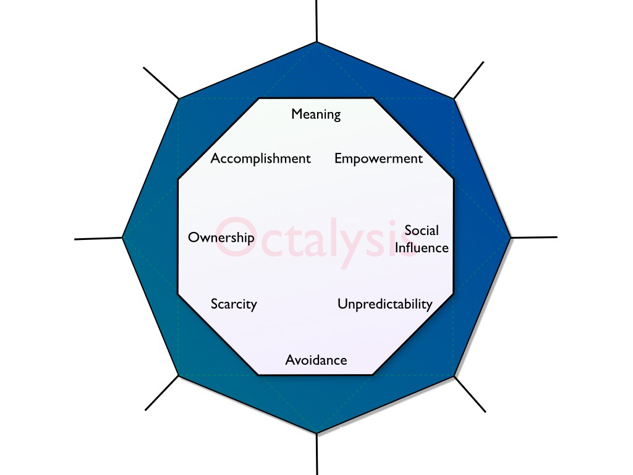
\includegraphics[width=400px, scale=1]{figuras/octalysisframework}
    \caption{Octalysis Framework}
    \label{fig:octalysisframework}
\end{figure}

Dessa forma, a seguir, serão explicadas as oito motivações básicas,
apontando quais são as suas respectivas técnicas, bem como
suas devidas explicações.

\subsubsection{Significado Épico e Chamado}
\label{sub:significadoepico}
Esta motivação básica está em torno de fazer com que o usuário sinta que
está fazendo algo épico e ajudando a sociedade, sendo altruísta com toda
a população. Fazendo-o acreditar que pode mudar algo muito importante
na vida de várias pessoas. Projetos Open Source são uma clara evidência
disto, onde o desenvolvedor trabalha e contribui para a comunidade, ajudando
todos.

Também entra nesta fase o fato de um jogador entrar no jogo e ganhar um
privilégio aparentemente muito valioso. Onde este acredita que teve uma
oportunidade que nenhum outro jogador, acreditando que ganhou a sorte de
principiante.

A seguir estão descritos as técnicas desta motivação básica:

\begin{enumerate}
    \item Narrativa: uma história que se inicia ao começar um determinado
        jogo, colocando o usuário dentro do enrendo e aplicando o contexto
        do "Modus Operants";
    \item Sorte de Principiante: sorte daquele que acredita que recebeu
        um benefício único e nenhum dos outros jogadores recebeu algo
        parecido;
    \item Lanche Grátis: técnica que atribui ou presenteia um dado usuário
        com algo que tem uma grande dificuldade de ser alcançado ou é
        caro e bastante dispendioso para o usuário.
        O ponto é que logo após o lanche, o game o incentiva a tomar
        algumas ações definidas;
    \item Elitismo: é a ação de aumentar e incentivar atitudes de orgulho
        de um grupo, fazendo com que os usuários destes sintam-se
        únicos e privilegiados, a fim de assegurar o orgulho do
        grupo inteiro, fazendo com que todos os integrantes sintam-se assim;
    \item Héroi da Humanidade: vem da técnica de que o jogador pode e deve
        ajudar a quem não consegue se ajudar, fazendo com que este tome
        atitudes e ações em prol de uma causa muito maior.
\end{enumerate}

\subsubsection{Motivação Desenvolvimento e Realização}
\label{sub:desenvolvimentoerealizacao}
A motivação básica de Desenvolvimento e Realização traz como base fazer
com que o jogador seja desafiado, que ele tenha metas a cumprir e que este
tem que desenvolver habilidades e fazer progressos para que o desafio
seja superado. É importante que nessa fase tenha recompensas e ganhos para
o jogador, como troféus, medalhas, emblemas, entre outros, para que o
usuário entenda que todo o esforço do desafio não foi em vão e que
teve um objetivo de recompensa por ele.

Exemplos desta motivação são os pontos, medalhas, rankings, tabelas de
classificação, emblemas, entre outros. Que já são largamente utilizados
em várias plataformas atualmente.

Alguns exemplos de técnicas de gamificação para a motivação básica
de Desafio e Realização estão listadas a seguir:

\begin{enumerate}
    \item Pontos: um esquema de pontos aplicado para mostrar o progresso
        de um jogador em qualquer ponto desejado do objeto a ser gamificado;
    \item Símbolos de conquista e realização: que são emblemas que podem
        ser utilizados como espécie de reconhecimento sobre dada
        atividade ou desafio que o usuário desempenhou. Estas podem ser
        medalhas, emblemas, troféus, uniformes, estrelas, entre outros.
    \item Tabelas de classificação: são tabelas que vão mostrar como o
        jogador se porta diante dos demais jogadores, como
        estão estes resultados e o quanto é necessário para alcançar
        algum determinado objetivo. Esta técnica pode ser aplicada através
        de rankings e tabelas.
    \item Barra de Progresso: permite que o usuário tenha uma clara visão
        e um bom feedback do quanto ele está cumprido ou cumpriu dentro
        de um determinado objetivo.
    \item Escolhas Óbvias: são caminhos diferentes onde o usuário tem que tomar
        uma certa decisão ou fazer uma escolha. Neste momento, o usuário tem um
        escolha óbvia dentre todas as demais. No momento que ele escolher a óbvia
        irá se achar inteligente por ter conseguido identificar algo e ter
        feito a escolha correta.
    \item Oasis no Deserto: é uma recompensa que está sugerida e presente logo
        após determinadas escolhas que o usuário pode fazer;
    \item Efeito Estrela do Rock: faz com que o usuário se sinta importante,
        com a ideia de que todos que estão na rede estão com vontade de interagir
        com ele, fazendo com que este se sinta importante, uma estrela do rock.
\end{enumerate}

\subsubsection{Motivação Empoderamento e Feedback}
\label{sub:empoderamentoefeedback}
A motivação básica de empoderamento e feedback é expressada quando os usuários
estão engajados em algum processo criativo e eles tem que tomar ações repentinas
e tentar diferentes combinações.

Para esta motivação básica o usuário não precisa apenas saber expressar
sua criatividade de várias maneiras, porém, além disso, precisa ser capaz
de ver os resultados das suas criações e seus respectivos feedbacks.

As técnicas que guiam esta motivação básica são as que estão listadas
a seguir:

\begin{enumerate}
    \item Escolhas significativas: esta técnica está em torno de fazer
        com que o usuário, mesmo com várias opções de montagem,
        tome ações corretas. O caminho correto não precisa ser exatamente o mesmo,
        pode ser um quebra-cabeças que você monta como desejar e no final
        consegue alcançar o objetivo esperado;
    \item Etapa desbloqueada: o usuário consegue ter acesso
        e utilizar novas funcionalidades, com novas possibilidades
        assim que uma etapa for concluída;
    \item Boosters: Itens temporários que o usuário tem alguma
        capacidade aumentada, com mais poder, durante um período
        determinado de tempo;
    \item Feedback instantâneo: característica que permite com que o usuário
        tenha uma resposta imediata das ações que ele escolheu fazer e proceder;
    \item Controle de tempo real: trazendo e possibilitando que o jogador
        possa controlar ações e opções de um determinado objetivo deste
        em tempo real;
    \item Chain Combos: um conjunto de ações que traz recompensa para o
        usuário, porém, quando feitos em seguida, como um combo, tem
        efeitos e ganhos maiores.
\end{enumerate}

\subsubsection{Motivação de Propriedade e Posse}
\label{sub:propriedadeeposse}
É a motivação que gira em torno de mostrar ao usuário e fazer com que
este acredite que ele tem posse sobre algo que está interagindo na
plataforma. Quando este, por exemplo, passa tanto tempo utilizando
ou personalizando algo que passa a sentir que aquele dado objeto
é propriedade dele.

Um exemplo que pode ser aplicado é a utilização de dinheiro e riquezas
virtuais, como moedas e bitcoins. De toda forma, um acumulo de riquezas
em geral contempla esta técnica.

\begin{enumerate}
    \item Construir do zero: faz com que o jogador sinta que ele está
        fazendo algo do início, e não que está recebendo algo que
        já está pronto para que este trabalhe;
    \item Coleção: transmite a ideia de um conjunto de itens que se todos
        estiverem juntos e reunidos, este irá se sentir completo.
    \item Pontos permutáveis: faz com que o usuário consiga utilizar
        seus pontos para adquirir algo que é caro por padrão;
    \item Monitor Attachment: faz com que o jogador sinta e tenha a
        sensação que é dono de algo devido ao longo monitoramento
        da atividade que está desempenhando.
    \item Efeito Alfred: este é definido quando os usuários
        sentem que um produto ou serviço é tão personalizado às
        suas próprias necessidades que não é possível fazer isso
        de nenhuma outra forma;
    \item Avatar: quando um jogador consegue criar um perfil que pode ser
        personalizado e permite com que este esteja próximo aos gostos e
        intenções do usuário.
\end{enumerate}

\subsubsection{Influência Social e Pertencimento}
\label{sub:influenciasocialepertencimento}
Esta motivação básica utiliza de elementos e fatos sociais de forma
a incentivar as pessoas à pensamentos e ações em grupos e comunidades,
de forma social.

Essa motivação básica vai de encontro com a característica de ver algum
amigo, conhecido ou familiar, que possui uma dado atributo ou expertise
em dada atividade. Você, rapidamente, analisando que não possui a mesma
habilidade, ou não no mesmo nível, se esforça e engaja para que consiga
alcançá-la e estar próximo de tal.

As técnicas que regem e que estão presentes na Influência Social e Pertencimento
são as listadas a seguir:

\begin{enumerate}
    \item Mentoria: no momento em que uma pessoa que possui mais experiência
        em um dado assunto e orienta aqueles que estão começando nesta, pode
        ser enquadrado nesta técnica;
    \item Vangloriar-se: mostrar e se apresentar aos demais usuários como
        alguém que possui uma determinada qualidade que é bem reconhecida
        por todos que estão em sua volta;
    \item Prateleira de Troféus: uma gama de troféus, recompensas e conquistas
        que estão bem aparentes para os demais usuários olharem e perceberem
        através de qualquer meio que foi estabelecido;
    \item Desafio em Grupo: dasafios que podem ser elaborados com ou dentro
        de um determinado grupo, que incentiva as pessoas a trabalharem
        em uma ação conjunta e não em algo isolado, com a utilização de atividade
        individual;
    \item Tesouro Social: são pontos, presentes e benefícios que podem ser atribuídos
        para você a partir de um determinado jogador ou amigo que se encontra dentro
        do círculo de amigos;
    \item Orgulho Social:  são ações pequenas, de pouco esforço, que auxiliam e contribuem
        para o convívio social, como eventos pequenos e pouco significativos,
        como um like em uma determinada rede social, ou um compartilhamento;
    \item Âncora de Conformidade: esta técnica possui base no que já temos ciência
        através de nossa cultura;
        influência social tem poder sobre nós.
    \item Water Cooler: esta técnica consiste em disponibilizar algum local
        aberto e comum para que as pessoas consigam escrever, expor e falar
        sobre fatos e atividades aleatórias, o qual agrada um determinado grupo.

\end{enumerate}

\subsubsection{Escassez e Impaciência}
\label{sub:escassexeimpaciencia}
Esta motivação leva o jogador a sentir-se ansioso e receoso com a espera de algo
que ele ainda não tem e para que consiga, tem que esperar por algum tempo.

Um exemplo bem utilizado deste ponto é a utilização dos games por meio de dinâmicas
agendadas, onde esses dizem ao usuário para retornar dentro de determinado tempo.
E caso o jogador não queira esperar por este tempo, deve utilizar algo que é caro
para este.

Um exemplo disto é a aplicação do Facebook quando iniciou, que tinha um início que não permitia
que todos utilizassem a plataforma, apenas se houvesse um convite por parte de um
determinado conhecido que já está dentro da base.

As técnicas que regem esta motivação básica são as seguir:

\begin{enumerate}
    \item Dangling: esta técnica deixa bem clara para o jogador que ele não pode
        ter algo que é bem gratificante. Que para ter deve esperar ou adquirir
        de uma forma cara e dispendiosa;
    \item Anchored Juxtaposition: esta técnica concede duas opções para o usuário.
        Uma delas custa dinheiro e a outra custa e exige bastante tempo e esforço
        por parte do usuário;
    \item Torture Breaks: esta técnica faz com que o usuário seja obrigado a esperar
        de qualquer forma para obter algo. Neste caso, existe um ponto em que
        se o usuário ficar por um período longo de tempo esperando esta ação
        utilizando o jogo, a gamifição já estará sendo bem aplicada;
    \item Evolved UI: fazer com que as pessoas tenham poucas opções no começo da
        trajetória, porém, com o seu desenvolvimento, estas opções vão aumentando.
\end{enumerate}

\subsubsection{Imprevisibilidade e Curiosidade}
\label{sub:imprevisibilidadeecuriosidade}
Esta motivação básica gira em torno de envolver o usuário com atitudes e ações que são
imprevisíveis, que o usuário não tem noção sobre o resultado que poderá receber.

Isto faz com que o usuário permaneça com a mente ocupada cogitando o que poderá
acontecer com o evento imprevisível.

As técnicas que guiam esta motivação básica são as listadas a sequir:

\begin{enumerate}
    \item Ovo de Pascoa: esta é uma notícia ou surpresa que agrada o usuário,
        que nasce de uma ação que não é esperada.
    \item Mystery Boxes: são recompensas que podem ser qualquer coisa
        logo após que alguma ação ou evento for concluído;
    \item Visual Storytelling: Fazer com que o usuário tenha informações
        advindas de formatos de livros e histórias
        visuais;
    \item Oracle Effect: esta técnica está em torno de fazer com que o
        jogador pense sobre o que está por vir, se será algo positivo ou não;
    \item Russian Roulette: é a prática onde de tempos em tempos algum dado ponto
        ou jogador deve ser penalizado.
\end{enumerate}

\subsubsection{Perda e Rejeição}
\label{sub:perdaerejeicao}
Esta motivação básica trabalha e se baseia em construir algo para que algo ruim não
aconteça com o jogador, ou seja, na prevenção de acontecimentos ruins.

São práticas como evitar que o jogador perca todas as atividades que desempenhou
até então, ou descobrir que todo o progresso foi em vão.

Estas atitudes motivam o usuário a executar determinados feitos com base no que
ele não quer que aconteça.

As seguintes técnicas ilustram como esses sentimentos são aplicados no meio:

\begin{enumerate}
    \item Reghtful Heritage: esta técnica está firmada em fazer com que o usuário
        acredite que algo é dele e pertence a ele, porém, depois de algum tempo,
        se o usuário não desempenhar determinadas ações, este terá este ponto
        perdido;
    \item Evanescente Opportunities: algo que não vai aparecer jamais
        caso o usuário não tome uma ação requerida rapidamente;
    \item Countdown Timers: são esquemas de contagem regressiva para determindas
        atividades, que tem um tempo máximo para se concluir;
    \item Status Wuo Sloth: tendência de mostrar ao jogador que este não irá evoluir ou melhorar se continuar
        a tomar atitudes como estão sendo tomadas;
    \item FOMO Ponch: este é um ponto muito forte da Motivação Básica 8, que tem como
        pretexto gerar no jogador um medo de perder, seja já qual for o que
        este adquiriu.
\end{enumerate}

\subsubsection{Left Brain and Right Brain}
\label{sub:leftright}
O Octalysis framework está dividido em duas partes, tais quais o Autor nomeia
de Left Brain e Right Brain, sendo que cada um destes é correspondente com qual lado do cérebro
as técnicas vão atuar. Cada motivação está posicionada em um dado local, que
representa um pensando de uma dada forma ou o contrário. Este posicionamento
da MB em cada lado representa qual lado do cérebro será utilizado.

A figura \ref{fig:octalysisleftright} ilustra esta divisão entre as técnicas.

\begin{figure}[h]
    \centering
    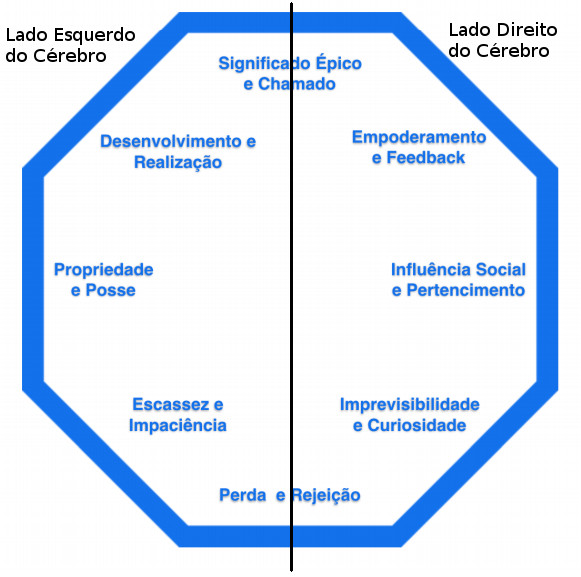
\includegraphics[width=400px, scale=1]{figuras/octalysisleftright}
    \caption{Left Brain and Right Brain}
    \label{fig:octalysisleftright}
\end{figure}

Pode ser visto que existem técnicas do lado direito e do lado esquerdo. As
motivações básicas do lado direito estão mapeadas também com o lado direito
do cérebro, o qual tem ligação com as atividades lógicas, de raciocínio lógico.
Já as motivações básicas do lado esquerdo represetam ações mais criativas,
sentimentais e imprevisíveis.

\subsubsection{White Hat and Black Hat}
\label{sub:whiteblack}
As motivações básicas estão muito ligadas à característica de pensamento e
sentimento que é gerado no jogador. Cada motivação básica gera um tipo de
sentimento e vontade diferente no usuário.

Estas diferenças são representadas pela parte superior, representadas
pela White Hat, que são sentimentos e motivações boas, que trazem
boas impressões para o jogador. A divisão é feita exatamente como
foi explicada na sessão \ref{sub:leftright}, porém, agora a
divisão é feita entre a parte superior ou inferior do framework.

Porém, a parte inferior do framework representa sentimentos ruins, que o jogador
vem a sentir no momento que participa e utiliza determinada MB. Já a
parte superior representa boas motivações, que ele chama de White Hat.

Todas essas disposições podem ser vistas na figura
\ref{fig:octalysiswhiteblack} a seguir.

\begin{figure}[h]
    \centering
    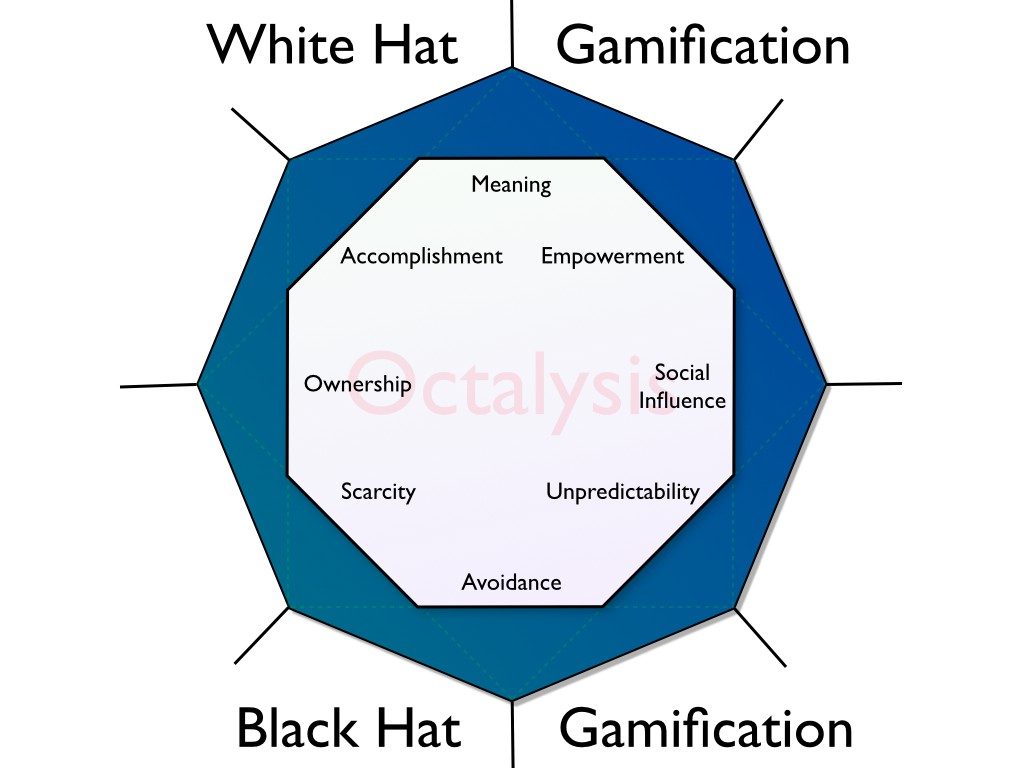
\includegraphics[width=400px, scale=1]{figuras/octalysiswhiteblack}
    \caption{White Hat and Black Hat}
    \label{fig:octalysiswhiteblack}
\end{figure}

\subsection{Fases da Gamificação}
\label{sub:fasesgamifição}
Todos os produtos que as pessoas utilizam na internet possuem diferentes
fases ao longo do seu ciclo de vida. Cada fase é reponsável por um tipo de contato diferente
do usuário com a interface e com a imersão em que este está submetido.

Cada fase representa um sentimento diferente, uma experiência diferente
e uma nova forma de se lidar com aqueles atributos referentes ao que está
em escopo no procedimento de interação com o produto propiciado.

Essas fases que cada projeto é submetido já são conhecidas e desenhadas. As fases
são quatro, bem claras e definidas. Elas são as seguintes:

\begin{enumerate}
    \item Descoberta;
    \item Reconhecimento;
    \item Construção;
    \item Fim de jogo.
\end{enumerate}

Essas fases circundam o ciclo de vida de um produto, desde o momento que este
é apresentado ao público até o momento que é deixado por ele.

A definição das fases será ilustrada claramente nos subcapítulos que virão a seguir.

\subsubsection{Descoberta}
\label{sub:descoperta}
É a fase onde o usuário não conhece sobre o produto, não tem noção de quais são
os
seus objetivos nem como pode utilizá-lo. Esta é a fase onde o usuário tem o primeiro
contato, onde percebe como este funciona, bem como seus conceitos e valores.

Um exemplo de descoberta é uma apresentação de uma página no facebook, onde,
o novo produto será demonstrado para grupos e nichos de interesse. A partir
de então, o usuário poderá passar a conhecer e utilizar o sistema.

Resumidamente, esta fase é reponsável por aprensentar o produto, fazer
com que os usuários o conheça.

\subsubsection{Reconhecimento}
\label{sub:reconhecimento}
Esta fase é reponsável por demonstrar ao usuário como o sistema se comporta.

Ela é essencial para que este entenda como o sistema funciona e o que cada
componente executa. Um exemplo bem conhecido desse procedimento é a utilização
de tutoriais e guias para novos usuários, no momento da sua chegada.

Ela termina quando o usuário está apto a continuar a utilizar o site sem
necessidade de aprender muitas outras novas ferramentas e funcionalidades.

Quando este está apto para tal, inicia-se a maior fase, onde o usuário
vai de fato entender e conhecer sobre o procedimento que está lidando.

\subsubsection{Construção}
\label{sub:constru_o}
Esta é a fase responsável pela real utilização do produto, onde as features
de fato serão utilizadas e irão agregar valor ao usuário.

Nesta parte o usuário já sabe e entende o papel de cada funcionalidade. Ele é capaz
de atingir os objetivos propostos. Aqui os recursos propostos serão utilizados
a depender na experiência e conexão do usuário com o produto.

Aqui tem que ser criados gatilhos para que mantenha o usuário constantemente utilizando
o sistema de acordo com o planejado.

\subsubsection{Fim de Jogo}
\label{sub:fim_de_jogo}
Toda aplicação desenvolvida passa pela fase de partida, onde é totalmente utilizada
e de alguma forma, o usuário a deixará.

Não necessariamente deixará de utilizar e participar do envolvimento total proposto pela
organização. Um exemplo disto é um jogo desenvolvido. Quando o primeiro jogo acabar, o
usuário passará pela fase de fim de jogo, que pode deixar o usuário motivado a se conectar
e adquirir a próxima versão do jogo que será lançada futuramente.

É importante que seja feito corretamente o desfeixo do produto para que uma linhagem seja
prosseguida.


Todas essas diretivas e fases que existem dentro do ciclo de vida de um produto
devem ser
tratadas de forma independente e diferente entre si. Agora pode-se indagar onde
a gamificação
entra neste processo, sendo que cada fase deve ser tratada de uma forma diferente pelo
usuário e, consecutivamente, por parte de quem está a oferecer o produto.

Assim, há a necessidade de que a gamificação também seja moldada conforme o objetivo de
cada fase a ser aplicada.

Dessa forma, cada fase implementada será pensada e avaliada para que seja possível
aplicação de um  projeto de gamificação. Cada fase terá um foco em motivações
básicas diferentes, que propiciarão uma experiência diferente para o usuário.

A figura \ref{fig:fasesoctalysis} ilustra um exemplo do como pode ser aplicado na
Rede Social About a gamificação ao longo das quatro fases.

\begin{figure}[h]
    \centering
    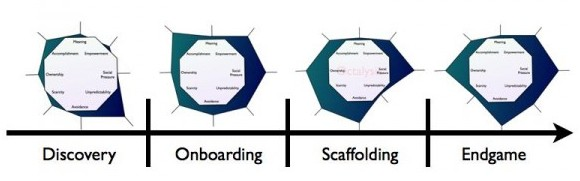
\includegraphics[width=400px, scale=1]{figuras/fasesoctalysis}
    \caption{Fases do Octalysis}
    \label{fig:fasesoctalysis}
\end{figure}

Como pode ser visto na figura \ref{fig:fasesoctalysis}, são projetados vários
desenhos e designs modificados e diferentes para cada fase. Cada uma destas
tem um pensamento e objetivo diferente.

Na fase de descoberta, pode ser visto que a motivação básica mais presente é
a imprevisão e a curiosidade. O que dá margem para que o usuário imagine diferentes
possibilidades sobre o produto.

No momento de uma propaganda, por exemplo, este lado do framework pode gerar uma
extrema curiosidade no usuário, o que fará com que ele fique motivado a procurar
e entender mais sobre o que está sendo anunciado.

Isto pode ser extremamente importante para conseguir capturar novos usuários.

Na segunda fase, em que o usuário vai conhecer sobre o produto, pode ser visto
que as fases relativas a desenvolvimento próprio e realização de si mesmo
são bem mais presentes.

Este ponto pode ser aplicado, pois o usuário irá se sentir realizado e inteligente
ao observar seu desenvolvimento próprio elevado. Isto irá gerar um prazer em fazê-lo
sentir o quanto pode ser bom em realizar as tarefas que a ele estão sendo designadas
no início do procedimento.

Na terceira fase é possível verificar que duas motivações básicas são muito presentes:

\begin{itemize}
    \item Motivação Básica Cinco: Influência e Dinâmica Social;
    \item Motivação Básica Seis: Escassez e Impaciência.
\end{itemize}


Para a Motivação Básica Cinco, isto deixa o usuário motivado ao utilizar o produto
por sentir que está exercendo uma alta influência social, que está envolvido em
uma dinâmica social que faz influência em outras pessoas.

Isto faz com que o usuário fique motivado a continuar engajado no processo, pois
este estará conseguindo perceber o quanto está sendo participativo no meio social
e que o produto está sendo proveitoso por fazê-lo se sentir socialmente influente
e participativo.


A segunda motivação básica vizualizada nesta fase, Escassez e Impaciência, acontece
pois é possível verificar que o usuário fique motivado a executar determinadas
tarefas baseado neste sentimento.

Esta o deixará preocupado com a questão de não cumprir corretamente os objetivos.
Esta fase é responsável por fazê-lo se sentir em um meio escasso caso não execute
os objetivos propostos.

Isto vai motivar o usuário e vai fazer com que faça o necessário para que não
sinta estes sentimentos.

A última fase, fim de jogo, também tem sua motivação básica predominante que
a guia. Esta é guiada pela Motivação Básica Oito: Perca e evitação.

Esta irá gerar um sentimento que faz o usuário se sentir mal. Este sentimento
envolve o fato de que o usuário pode perder todo o processo que foi executado.



Este é um sentimento ruim. Sentimento qual o usuário não deseja sentir. Para tanto
ele se esforçará a fim de não presenciar as experiências que são submetidas.

Como pode ser visto, estes procedimentos de cada fase são extremamente aplicáveis
e úteis para que o usuário tenha várias experiências ao longo do clico de vida do
produto. O que propiciará uma experiência muito mais agradável.

Dessa forma, serão desenhados quatro frameworks diferentes para a Rede Social About.
Uma para cada fase diferente do produto, onde serão estudadas separadamente para
aplicá-las e possibilitar uma boa experiência para o usuário.

\subsection{Octalysis Strategy Dashboard}
\label{sec:octalysisdashborad}
O framework octalysis oferece suporte para a construção de um projeto de gamificação
bem estruturado e baseado em necessidades do domínio do problema.

Este suporte se trata do Octalysis Strategy Dashboard, o qual pode ser analisado
 as
estretégias de mercado, perspectiva do usuário, intenções desejadas para a gamificação,
mecanismos de feedback e incentivos.

Existem processos sistematizados para estabelecer cada fase e como será dado o
resultado da gamificação.

Para este trabalho, serão utilizados estes procedimentos sistematizados.

Para ilustrar a metodologia de estratégia do octalysis dashboard, será representada
a figura a seguir, que contém a metodologia e a formalização da sua construção.

A seguir serão descritos subcapítulos, que retratarão o papel e a utilidade de
cada
componente.


 \begin{figure}[h]
     \centering

     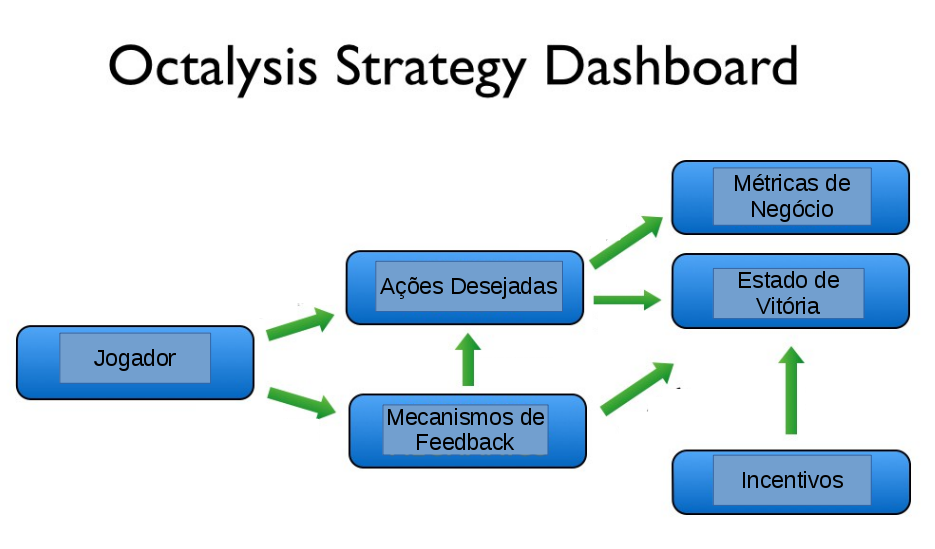
\includegraphics[width=450px, scale=1]{figuras/dashboard}
     \caption{Octalysis Strategy Dashboard}

     \label{fig:dashboard}
 \end{figure}

\subsubsection{Business Metrics}
\label{sub:business_metrics}
As métricas de negócio, em português, são termos quantitativos que podem ser utilizados
para ter um número palpável sobre como está um determinado ponto do projeto de gamificação
que teve como o objetivo de ser atacado.

Essas métricas, irão auxiliar a verificarmos o quanto a aplicação da gamificação
 foi eficaz ou
não dentro de um determinado objetivo.

Alguns exemplos de técnica de gamificação que serão utilizadas estão a seguir:

\begin{itemize}
    \item Aumentar o número de seguidores dos usuários prêmio
    \item Aumentar o número de vendas de um livro sobre o produto
    \item Aumentar o número de inscritos na rede social
    \item Aumentar a quantidade de acessos diários
    \item Aumentar os seguidores inscritos
    \item Aumentar os usuários que compartilham conteúdos pelas redes sociais
    \item Aumentar a quantidade de curtidas em determinado post
\end{itemize}

Estes exemplos de métricas serão submetidos à Rede Social About antes da apresentação da
gamificação. E assim que determinada técnica for utilizada, será então executada
 uma
segunda medição, que propiciará analisar as diferenças entre os resultados obtidos.

\subsubsection{Define User Types}
\label{sub:define_user_types}
Este ponto do dashboard, para definir os tipos dos usuários, é responsável por conseguir
elaborar e definir quais são os tipos de usuários que serão almejados e trabalhados, quando
falamos sobre gamificação.

Esta fase é um processo de definição de nicho sobre onde a gamificação vai atuar, quanto a
usuários, dentro da Rede Social About? Quais serão os passos utilizados para que este público
seja atingindo?

Alguns exemplos de tipos de usuário se encontram a seguir:

\begin{itemize}
    \item Companhias que desejam que seus trabalhadores atinjam determinadas métricas
        ao fim de cada mês;
    \item Educadores e políticos que querem utilizar conhecimento para criar impactos
        sociais;
    \item Indivíduos que são apaixonados por gamificação, games e desenvolvimento próprio.
\end{itemize}

Desta maneira, será possível realizar um projeto de gamificação focado ao definir o tipo
de usuários. Pois, a partir daí, será possível identificar quais caminhos são mais vantajasos
quanto a escolha das motivações básicas que serão utilizadas ao longo das quatro fases.

\subsubsection{Define Desired Actions}
\label{sub:define_desired_actions}
A definição das ações desejadas são todas as iniciativas tomadas pelo usuário que o levam a caminhar para
o Win Stade(Estado de Vitória), seja ela em qual fase for. Sendo assim, a Rede Social
About terá alguns pontos que serão definidos como os desejados. Estes serão desenhados
até que o estado de vitória seja definido. Assim, para as quatro fases serão definidas
ações diferentes. Alguns exemplos de ações que podem ser escolhidas serão apresentadas
a seguir.

Ações na fase da descoberta:
\begin{itemize}
    \item Conhecer a Rede Social About;
    \item Clicar no link da Rede Social About
    \item Conhecer as features oferecidas pela Rede Social
\end{itemize}


Ações na fase de reconhecimento do projeto:
\begin{itemize}
    \item Executar o tutorial de uso da About;
    \item Compartilhar a Rede Social About com os amigos
    \item Adicionar foto e email na network
    \item Permitir a inscrição na lista de email
\end{itemize}

Já para a fase de construção do projeto, os seguintes pontos podem ser um
exemplo:

\begin{itemize}
    \item Fazer login diariamente na network
    \item Abrir semanalmente os emails enviados pela network
    \item Compartilhar abouts com os amigos
    \item Participar de grupos no facebook sobre a rede social about
    \item Adquirir a versão prêmio da rede social about
    \item Inscrever em grupos de discussão sobre a rede social about
    \item Escrever mais de um about diariamente
    \item Votar em mais de vinte abouts diários
\end{itemize}

Por fim, na fase de fim de jogo, alguns exemplos de construção podem ser dados.
Eles são os seguintes:
\begin{itemize}
    \item Se tornar contribuidor da Rede Social About;
    \item Fazer parte da equipe de desenvolvedores da About
    \item Propor melhorias para a about
    \item Tornar-se moderador dos abouts
\end{itemize}

Estes exemplos ajudam e esclarecer como os objetivos podem ser alcançados. Elas
definem um nível de
granularidade maior.

\subsubsection{Define Feedback Mechanics}
\label{sub:define_feedback_mechanics}
A definição de mecanismos de feedback são extremamente importantes para a experiência do usuário
com a network. Este é responsável por ilustrar e deixar bem claro para o usuário
, como ele está
prosseguindo no desenvolvimento do projeto.

Atualmente os usuários tem requirido feedbacks constantes, em tempo real, para as suas ações
realizadas. Sendo assim, é necessário que existam esses gatilhos em vários pontos da
Rede Social About e que o usuário possa entender rapidamente.

A seguir estão alguns exemplos de como podem ser esclarecidos esses feedbacks para o usuário:

\begin{itemize}
    \item Countdown Timers
    \item Desbloquear conteúdo da página
    \item Status de progresso na sidebar
    \item Verificação de qual era a melhor escolha
    \item Vídeo embutido
    \item Barra de pontos de status
    \item Certificados
    \item Medalhas
    \item Gráficos de desempenho
\end{itemize}

Assim, com exemplos dessa maneira, é possível que o usuário verifique o quanto suas atividades estão
sendo aproveitadas.

\subsubsection{Incentives And Rewards}
\label{sub:incentives_and_rewards}
O sistema de incentivos e recompensas fecham o ciclo do dashboard, que fazem com que
os usuários se sintam motivados a alcançar cada estado de vitória. Eles ajudam a
indicar
o quanto ainda falta para que o estado seja almejado.

\begin{itemize}
    \item Status Points
    \item Símbolos de vitórias
    \item Conhecer os desenvolvedores da about
    \item Ter acesso a arquivos confidenciais
    \item Descontos nos produtos
\end{itemize}

\subsubsection{Objetos de Gamificação}
\label{sec:objetodegamificacao}
Os objetos de gamificação serão os pontos da rede social em que será aplicado o framework,
com os objetivos de atingir alguma meta de negócio.

Os objetivos de gamificação são os seguintes:

\begin{itemize}
    \item Fazer com que o usuário escreva mais abouts;
    \item Fazer com que o usuário julgue mais abouts;
    \item Fazer com que o usuário convide amigos que não estão cadastrados na about;
\end{itemize}

